\documentclass[11pt,a4paper,titlepage]{article}
\usepackage[a4paper]{geometry}
\usepackage[utf8]{inputenc}
\usepackage[english]{babel}
\usepackage{lipsum}

\usepackage{amsmath, amssymb, amsfonts, amsthm, mathtools, physics}
% mathtools for: Aboxed (put box on last equation in align envirenment)
\usepackage{microtype} %improves the spacing between words and letters
\usepackage{listings} %insert codeblocks
\usepackage{graphicx} %package to manage images
\usepackage{float} %force figure placement
\graphicspath{ {Code/} }
\usepackage{minted} %package to manage code blocks
\usepackage{caption} %captions of the figures
\usepackage{subcaption} %captions of the subfigures



%%%%%%%%%%%%%%%%%%%%%%%%%%%%%%%%%%%%%%%%%%%%%%%%%%
%    SECTIONS
%%%%%%%%%%%%%%%%%%%%%%%%%%%%%%%%%%%%%%%%%%%%%%%%%%
\usepackage{titlesec}
\usepackage{sectsty}
%%%%%%%%%%%%%%%%%%%%%%%%
%set section enumerator to arabic number (see footnotes markings alternatives)
\renewcommand\thesection{Question \arabic{section}} %define sections numbering
\renewcommand\thesubsection{\arabic{section}.\alph{subsection}} %number.letter
\renewcommand\thesubsubsection{\arabic{section}.\alph{subsection}.\roman{subsubsection}} %tabbed roman numeral

%define new section style
\newcommand{\mysection}{
\titleformat{\section} [runin] {\usefont{OT1}{lmss}{b}{n}} 
{\thesection} {3pt} {} } 



%%%%%%%%%%%%%%%%%%%%%%%%%%%%%%%%%%%%%%%%%%%%%%%%%%
%		Shortcuts
%%%%%%%%%%%%%%%%%%%%%%%%%%%%%%%%%%%%%%%%%%%%%%%%%%
\newcommand{\R}{\mathbb{R}}



\makeatletter
\let\reftagform@=\tagform@
\def\tagform@#1{\maketag@@@{(\ignorespaces\textcolor{red}{#1}\unskip\@@italiccorr)}}
\renewcommand{\eqref}[1]{\textup{\reftagform@{\ref{#1}}}}
\makeatother
\usepackage{hyperref}
\hypersetup{colorlinks=true}

%%%%%%%%%%%%%%%%%%%%%%%%%%%%%%%%%%%%%%%%%%%%%%%%%%
%% PREPARE TITLE
%%%%%%%%%%%%%%%%%%%%%%%%%%%%%%%%%%%%%%%%%%%%%%%%%%
\title{CS 229: Machine Learning\\
Problem Set $2$}
\author{William Ma}
\date{\today}
%%%%%%%%%%%%%%%%%%%%%%%%%%%%%%%%%%%%%%%%%%%%%%%%%%



\begin{document}
\maketitle

\section{}{
\subsection{}{
\quad Given $K(x^{(i)}, x^{(j)}) = K_1(x^{(i)}, x^{(j)}) + K_2(x^{(i)}, x^{(j)})$, where $K_1$ and $K_2$ are kernels, $K$ is a kernel because it's kernel matrix is symmetric by the following
\begin{align*}
	K(x^{(i)}, x^{(j)}) &= K_{ij}
    \\ &= K_1(x^{(i)}, x^{(j)}) + K_2(x^{(i)}, x^{(j)})
    \\ &= K_1(x^{(j)}, x^{(i)}) + K_2(x^{(j)}, x^{(i)})
    \\ &= K_{ji} = K(x^{(j)}, x^{(i)})
\end{align*}
Additionally, for any vector $z$.
\begin{align*}
	z^TKz &= z^T(K_1+K_2)z
    \\ &= z^TK_1z + z^TK_2z
	\\ &\geq 0
\end{align*}
Thus, $K$ is a positive semidefinite (PSD) matrix. Since the kernel matrix is PSD, by the Mercer theorem, $K$ is also a valid kernel.
}\label{prob:1a}
%%% END SUBSECTION 1 %%%%%%%%%%%%%%%%%%%%%%%%%%%%%%%%%%%%%%
\subsection{}{
\quad Given $K(x^{(i)}, x^{(j)}) = K_1(x^{(i)}, x^{(j)}) - K_2(x^{(i)}, x^{(j)})$, where $K_1$ and $K_2$ are kernels, $K$ is not a kernel. It is obvious that the proof for $K$ is similar to the one for Problem \ref{prob:1a} except it is subtraction of two kernels instead of addition. Thus, if $z^TK_1z \leq z^TK_2z$, $z^TKz \leq 0$, causing $K$ to no longer be PSD.
}\label{prob:1b}
%%% END SUBSECTION 2 %%%%%%%%%%%%%%%%%%%%%%%%%%%%%%%%%%%%%%
\subsection{}{
\quad Given $K(x^{(i)}, x^{(j)}) = aK_1(x^{(i)}, x^{(j)})$, where $K_1$ is a kernel and $a\in\R$, $K$ is a kernel because it's kernel matrix is symmetrical as follows.
\begin{align*}
	K(x^{(i)}, x^{(j)}) &= K_{ij}
    \\ &= aK_1(x^{(i)}, x^{(j)})
    \\ &= aK_1(x^{(j)}, x^{(i)})
    \\ &= K_{ji} = K(x^{(j)}, x^{(i)})
\end{align*}
Additionally, for any vector $z$,
\begin{align}
	z^TKz &= z^T(aK_1)z
    \\ &= a(z^TK_1z)
	\\ &\geq 0.
\end{align}
Thus, $K$ is PSD. Since $K$ is PSD, by the Mercer theorem, $K$ is a valid kernel.
}\label{prob:1c}
%%% END SUBSECTION 3 %%%%%%%%%%%%%%%%%%%%%%%%%%%%%%%%%%%%%%
\subsection{}{
\quad Given $K(x^{(i)}, x^{(j)}) = -aK_1(x^{(i)}, x^{(j)})$, where $K_1$ is a kernel and $a\in\R$, $K$ is not a kernel because, for any vector $z$, 
\begin{align*}
	z^TKz &= z^T(-aK_1)z
    \\ &= -a(z^TK_1z)
    \\ \leq 0.
\end{align*}
Thus, $K$ is not PSD and, thus, not a valid kernel.
}\label{prob:1d}
%%% END SUBSECTION 4 %%%%%%%%%%%%%%%%%%%%%%%%%%%%%%%%%%%%%%
\subsection{}{
\quad Given $K(x, z) = K_1(x, z) K_2(x, z)$, where $K_1$ and $K_2$ are kernels, $K$ is a kernel. We can consider 
\begin{align}
	K_1(x, z) &= \sum_{i=1}^m a_i(x)^T a_i(z)
    \\K_2(x, z) &= \sum_{j=1}^m b_j(x)^T b_j(z)
\end{align}
Thus, we can rewrite $K$ as
\begin{align*}
	K(x, z) &= \sum_{i=1}^m a_i(x)^T a_i(z) \sum_{j=1}^m b_j(x)^T b_j(z)
    \\ &= \sum_{i=1}^m \sum_{j=1}^m a_i(x)^T a_i(z) b_j(x)^T b_j(z)
    \\ &= \sum_{i=1}^m \sum_{j=1}^m c_{ij}(x)^T c_{ij}(z),
\end{align*}
where $c_{ij}(x) = a_i(x) b_j(x)$. Thus, since $K$ can be rewritten as an inner product of two functions $c$, by the definition of kernels, $K$ is a kernel.
}\label{prob:1e}
%%% END SUBSECTION 5 %%%%%%%%%%%%%%%%%%%%%%%%%%%%%%%%%%%%%%
\subsection{}{
\quad Given $K(x, z) = f(x)f(z)$, $K$ is a kernel because $f(x)f(z)$ can be rewritten as $\phi(x)^T\phi(z)$, which would lead to $K=\phi(x)^T\phi(z)$, the definition of kernels.
}\label{prob:1f}
%%% END SUBSECTION 6 %%%%%%%%%%%%%%%%%%%%%%%%%%%%%%%%%%%%%%
\subsection{}{
\quad Given $K(x, z) = K_3(\phi(x), \phi(z))$, where $K_3$ is a kernel, $K$ is a kernel because, since the matrix $K$ from the set $\{x^{(1)},\ldots,x^{(m)}\}$ is PSD, then it is also PSD from the set $\{\phi(x^{(1)}),\ldots,\phi(x^{(m)})\}$.
}\label{prob:1g}
%%% END SUBSECTION 7 %%%%%%%%%%%%%%%%%%%%%%%%%%%%%%%%%%%%%%
\subsection{}{
\quad Given $K(x, z) = p(K_3(x,z))$, where p(x) is a polynomial over $x$ with positive coefficients, $K$ is a kernel because kernel addition (\ref{prob:1a}), kernel constant multiplication (\ref{prob:1c}), kernel kernel multiplication (\ref{prob:1e}), and kernels that return constants (\ref{prob:1f}) all are valid kernels. Thus, $K$ is a valid kernel.
}\label{prob:1h}
%%% END SUBSECTION 8 %%%%%%%%%%%%%%%%%%%%%%%%%%%%%%%%%%%%%%
}\label{problem 1}
%%% END SECTION 1 %%%%%%%%%%%%%%%%%%%%%%%%%%%%%%%%%%%%%%%%%	
\section{}{
\quad We can apply the "kernel trick" that we used in SVM to perceptrons for perceptrons to work in the feature space $\phi$. We are able to do so by (implicitly) representing the parameters $\theta$ as a linear combination of the inputs it as seen as such, $\theta^{(i)} = \sum_{j=1}^i \beta_j \phi(x^{(j)})$. Before we can use $h_\theta(x) = g(\theta^Tx)$, we have to solve $\theta^T\phi(x^{(j)})$ as follows
\begin{align*}
	\theta^T\phi(x^{(j)}) &= \sum_{j=1}^i \beta_j \phi(x^{(j)}) x
    \\ &= \sum_{j=1}^i \beta_j K(\phi(x^{(j)}), x)
\end{align*}
Thus, we can make a new prediction on a new input $\phi(x^{(i+1)})$ by computing the following
\begin{align*}
	h_{\theta^{(i)}}(x^{(i+1)}) &= g(\theta^{{(i)}^T} \phi(x^{(i+1)}))
    \\ &= g(\sum_{j=1}^{i} \beta_j K(\phi(x^{(j)}), \phi(x^{(i+1)}))
\end{align*}
Finally, we'd update the the parameters to include $x^{(i)}$ and $y^{(i)}$ by adding the weight $\beta_i$ and letting $\beta_i = \alpha 1\{\theta{(i)^T}\phi(x^{(i+1)})y^{(i+1)}<0\} y^{(i+1)}$.
}\label{problem 2}
%%% END SECTION 2 %%%%%%%%%%%%%%%%%%%%%%%%%%%%%%%%%%%%%%%%%
\section{}{
\subsection{}{
\quad The following is the implementation of the training and testing of the multinomial naive Bayes classifier with Laplace smoothing.
\begin{minted}{matlab}
function [phi_y, phi_spam, phi_not_spam] = nb_train(filename)

[spmatrix, tokenlist, trainCategory] = readMatrix(filename);

trainMatrix = full(spmatrix);
numTrainDocs = size(trainMatrix, 1);
numTokens = size(trainMatrix, 2);

% trainMatrix is now a (numTrainDocs x numTokens) matrix.
% Each row represents a unique document (email).
% The j-th column of the row $i$ represents the number of times the j-th
% token appeared in email $i$. 

% tokenlist is a long string containing the list of all tokens (words).
% These tokens are easily known by position in the file TOKENS_LIST

% trainCategory is a (1 x numTrainDocs) vector containing the true 
% classifications for the documents just read in. The i-th entry gives the 
% correct class for the i-th email (which corresponds to the i-th row in 
% the document word matrix).

% Spam documents are indicated as class 1, and non-spam as class 0.
% Note that for the SVM, you would want to convert these to +1 and -1.


% YOUR CODE HERE

numSpam = 0;

phi_spam_numerators = zeros(numTokens, 1);
phi_spam_denominators = zeros(numTokens, 1);

phi_not_spam_numerators = zeros(numTokens, 1);
phi_not_spam_denominators = zeros(numTokens, 1);


% Laplace smoothing
phi_spam_numerators(:) = 1;
phi_not_spam_numerators(:) = 1;
phi_spam_denominators(:) = numTokens;
phi_not_spam_denominators(:) = numTokens;

for i = 1:numTrainDocs
    y = trainCategory(i);
    x_i = trainMatrix(i,:);
    if y == 1
        numSpam = numSpam + 1;
    end
    
    docNumWords = 0;
    
    for j = 1:numTokens
        x_ij = x_i(j);
        docNumWords = docNumWords + x_ij;
        if y == 1
            phi_spam_numerators(j) = phi_spam_numerators(j) + x_ij;
        else
            phi_not_spam_numerators(j) = phi_not_spam_numerators(j) + x_ij;
        end
    end
    
    if y == 1
        phi_spam_denominators(:) = phi_spam_denominators(:) + docNumWords;
    else
        phi_not_spam_denominators(:) = phi_not_spam_denominators(:) + docNumWords;
    end
end

phi_y = numSpam / numTrainDocs;
phi_spam = phi_spam_numerators ./ phi_spam_denominators;
phi_not_spam = phi_not_spam_numerators ./ phi_not_spam_denominators;

clearvars numSpam phi_spam_numerators phi_spam_denominators
clearvars phi_not_spam_numerators phi_not_spam_denominators
clearvars docNumWords i j numTrainDocs spmatrix tokenlist x_i x_ij y


function [error] = nb_test(filename, phi_y, phi_spam, phi_not_spam)

[spmatrix, tokenlist, category] = readMatrix(filename);

testMatrix = full(spmatrix);
numTestDocs = size(testMatrix, 1);
numTokens = size(testMatrix, 2);

% Assume nb_train.m has just been executed, and all the parameters computed/needed
% by your classifier are in memory through that execution. You can also assume 
% that the columns in the test set are arranged in exactly the same way as for the
% training set (i.e., the j-th column represents the same token in the test data 
% matrix as in the original training data matrix).

% Write code below to classify each document in the test set (ie, each row
% in the current document word matrix) as 1 for SPAM and 0 for NON-SPAM.

% Construct the (numTestDocs x 1) vector 'output' such that the i-th entry 
% of this vector is the predicted class (1/0) for the i-th  email (i-th row 
% in testMatrix) in the test set.
output = zeros(numTestDocs, 1);

%---------------
% YOUR CODE HERE
for i = 1:numTestDocs
    prob_spam = log(phi_y);
    prob_not_spam = log(1 - phi_y);
    for j = 1:numTokens
        curr_val = testMatrix(i, j);
        prob_spam = prob_spam + curr_val * log(phi_spam(j));
        prob_not_spam = prob_not_spam + curr_val * log(phi_not_spam(j)); 
    end
    if prob_spam >= prob_not_spam
        output(i) = 1;
    else
        output(i) = 0;
    end
end
%---------------


% Compute the error on the test set
y = full(category);
y = y(:);
error = sum(y ~= output) / numTestDocs;

%Print out the classification error on the test set
fprintf(1, 'Test error: %1.4f\n', error);
\end{minted}
}\label{prob:3a}
%%% END SUBSECTION 1 %%%%%%%%%%%%%%%%%%%%%%%%%%%%%%%%%%%%%%
\subsection{}{
\quad Using the following code, we got the 5 tokens most indicative of the SPAM class to be links, 'spam', 'unsubscrib', 'ebai', and 'valet.' 
\begin{minted}{matlab}

% Read in token list
filename = 'TOKENS_LIST';
delimiter = ' ';
formatSpec = '%f%s%[^\n\r]';
fileID = fopen(filename,'r');
dataArray = textscan(fileID, formatSpec, 'Delimiter', delimiter, 'MultipleDelimsAsOne', true);
fclose(fileID);
tokens = dataArray{:, 2};
clearvars filename delimiter formatSpec fileID dataArray ans;

% Train NB Classifier
[phi_y, phi_spam, phi_not_spam] = nb_train('MATRIX.TRAIN');

% Calculate predictive power of tokens
ratio = phi_spam ./ phi_not_spam;
[sortedRatio,sortingIndices] = sort(ratio,'descend');
topFiveTokens = tokens(sortingIndices(1:5))

clear
\end{minted}
}\label{prob:3b}
%%% END SUBSECTION 2 %%%%%%%%%%%%%%%%%%%%%%%%%%%%%%%%%%%%%%
\subsection{}{
\quad Using the following code, we got errors 3.87\%, 2.62\%, 2.62\%, 1.87\%, 1.75\%, and 1.63\% for training sets sizes 50, 100, 200, 400, 800, and 1400, respectively.
\begin{minted}{matlab}
numTrainDocs = [50, 100, 200, 400, 800, 1400];

% Create file name
for num = numTrainDocs
    filename = strcat('MATRIX.TRAIN.', int2str(num));

    % Train NB Classifier
    [phi_y, phi_spam, phi_not_spam] = nb_train(filename);

    % Test NB Classifier
    nb_test('MATRIX.TEST', phi_y, phi_spam, phi_not_spam);
end

clear
\end{minted}
}\label{prob:3c}
%%% END SUBSECTION 3 %%%%%%%%%%%%%%%%%%%%%%%%%%%%%%%%%%%%%%
\subsection{}{
\quad The following code is our implementation of the SVM using a radial basis kernel and stochastic gradient descent.
\begin{minted}{matlab}
function [average_alpha, Xtrain, squared_X_train, num_train] = svm_train(num_train)

% Before using this method, set num_train to be the number of training
% examples you wish to read.

[sparseTrainMatrix, tokenlist, trainCategory] = ...
    readMatrix(sprintf('MATRIX.TRAIN.%d', num_train));

% Make y be a vector of +/-1 labels and X be a {0, 1} matrix.
ytrain = (2 * trainCategory - 1)';
Xtrain = 1.0 * (sparseTrainMatrix > 0);

numTrainDocs = size(Xtrain, 1);
numTokens = size(Xtrain, 2);

% Xtrain is a (numTrainDocs x numTokens) sparse matrix.
% Each row represents a unique document (email).
% The j-th column of the row $i$ represents if the j-th token appears in
% email i.

% tokenlist is a long string containing the list of all tokens (words).
% These tokens are easily known by position in the file TOKENS_LIST

% trainCategory is a (1 x numTrainDocs) vector containing the true 
% classifications for the documents just read in. The i-th entry gives the 
% correct class for the i-th email (which corresponds to the i-th row in 
% the document word matrix).

% Spam documents are indicated as class 1, and non-spam as class 0.
% For the SVM, we convert these to +1 and -1 to form the numTrainDocs x 1
% vector ytrain.

% This vector should be output by this method
average_alpha = zeros(numTrainDocs, 1);

%---------------
% YOUR CODE HERE

tau = 8;
steps = 40 * num_train;
lambda = 1 / (64 * num_train);
alpha = zeros(numTrainDocs, 1);

squared_X_train = sum(Xtrain.^2, 2);
middle_matrix = Xtrain * Xtrain';
K = full(exp(-(repmat(squared_X_train, 1, num_train) + ...
    repmat(squared_X_train', num_train, 1) + 2 * middle_matrix)/ (2 * tau^2)));

for i = 1:steps
    stepsize = 1/sqrt(i);
    index = ceil(rand * num_train);
    margin = ytrain(index) * K(:, index)' * alpha;
    g = -(margin < 1) * ytrain(index)* K(:, index)...
        + lambda * K(:, index) * alpha(index);
    alpha = alpha - stepsize * g;
    average_alpha = average_alpha + alpha;
end

average_alpha = average_alpha ./ steps;
%---------------


function [error] = svm_test(average_alpha, Xtrain, squared_X_train, num_train)

[sparseTestMatrix, tokenlist, testCategory] = readMatrix('MATRIX.TEST');

% Make y be a vector of +/-1 labels and X be a {0, 1} matrix.
Xtest = 1.0 * (sparseTestMatrix > 0);
ytest = (2 * testCategory - 1)';

numTestDocs = size(sparseTestMatrix, 1);
numTokens = size(sparseTestMatrix, 2);

% Assume svm_train.m has just been executed, and the model trained
% by your classifier is in memory through that execution. You can also assume 
% that the columns in the test set are arranged in exactly the same way as for the
% training set (i.e., the j-th column represents the same token in the test data 
% matrix as in the original training data matrix).

% Write code below to classify each document in the test set (ie, each row
% in the current document word matrix) as 1 for SPAM and 0 for NON-SPAM.

% Note that the predict function for LIBLINEAR uses the sparse matrix 
% representation of the document word  matrix, which is stored in sparseTestMatrix.
% Additionally, it expects the labels to be dimension (numTestDocs x 1).

% Construct the (numTestDocs x 1) vector 'predictions' such that the i-th
% entry of this vector is positive if the predicted class is 1 and negative if
% the predicted class is -1 for the i-th email (i-th row in Xtest) in the test
% set.
predictions = zeros(numTestDocs, 1);

%---------------
% YOUR CODE HERE

tau = 8;
num_test = numTestDocs;
squared_X_test = sum(Xtest.^2, 2);
middle_matrix = Xtest * Xtrain';
K = full(exp(-(repmat(squared_X_test, 1, num_train) + ...
    repmat(squared_X_train', num_test, 1) + 2 * middle_matrix)/ (2 * tau^2)));
predictions = K * average_alpha;
%---------------

% Compute the error on the test set
error = sum(ytest .* predictions <= 0) / numTestDocs;
fprintf(1, 'Test error for SVM: %1.4f\n', error);
\end{minted}
\quad Using the following code, we got errors 9.88\%, 0.63\%, 0.37\%, 0.25\%, 0\%, and 0\% for training sets sizes 50, 100, 200, 400, 800, and 1400, respectively.
\begin{minted}{matlab}
numTrainDocs = [50, 100, 200, 400, 800, 1400];

% Create file name
for num = numTrainDocs
    % Train NB Classifier
    [average_alpha, Xtrain, squared_X_train, num_train] = svm_train(num);

    % Test NB Classifier
    svm_test(average_alpha, Xtrain, squared_X_train, num);
end

clear
\end{minted}
}\label{prob:3d}
%%% END SUBSECTION 4 %%%%%%%%%%%%%%%%%%%%%%%%%%%%%%%%%%%%%%
\subsection{}{
Excluding the data set with only 50 training examples, it is obvious that SVM is better for this data set than naive Bayes.
}\label{prob:3e}
%%% END SUBSECTION 5 %%%%%%%%%%%%%%%%%%%%%%%%%%%%%%%%%%%%%%
}\label{problem 3}
%%% END SECTION 3 %%%%%%%%%%%%%%%%%%%%%%%%%%%%%%%%%%%%%%%%%
\section{}{
\subsection{}{
\begin{proof}
Given two hypothesis classes $H_1$ and $H_2$ that satisfy $H_1 \subset H_2$, we let $VC(H_1) = d$. Since $H_1$ is a subset of $H_2$, $H_2$ can also shatter a set of $d$ points. Further, $H_2$ may contain hypotheses that can shatter sets containing more than $d$ points. Thus, $VC(H_2) \geq VC(H_1)$.
\end{proof}
}\label{prob:4a}
%%% END SUBSECTION 1 %%%%%%%%%%%%%%%%%%%%%%%%%%%%%%%%%%%%%%
\subsection{}{
\begin{proof}
Given two hypothesis classes $H_1^{(0)}$ and $H_2$ where $H_1^{(0)} = H_2 \cup \{h_1,\ldots, h_k\}$, we let $VC(H_2) = d$. 
\quad We first consider the case where $k=1$. We let $h_1 = h_1^{(0)}$ be the hypothesis that $H_2^{(0)}$ needs to shatter a set of $d+1$ points. Then, we let $H_2^{(1)} = H_1^{(0)}$ and $H_1^{(1)} = H_2^{(1)} \cup \{h_1^{(1)}\}$, where $h_1^{(1)}$ is the hypothesis needed for $H_2^{(1)}$ to shatter a set of $d+2$ points. We can repeat this process $k$ times to get the result $H_1 = H_2 \cup \{h_1,\ldots, h_k\}$, where $VC(H_1) = VC(H_2) + k$. 
\quad However, we also consider the cases where, on the $i$-th step, the additional hypothesis $h_1^{(i)}$ is not the one needed for $H_2^{(i)}$ to shatter a set of $d+(i+1)$ points. Thus, we change $VC(H_1) = VC(H_2) + k$ to $VC(H_1) \leq VC(H_2) + k$.
\end{proof}
}\label{prob:4b}
%%% END SUBSECTION 2 %%%%%%%%%%%%%%%%%%%%%%%%%%%%%%%%%%%%%%
\subsection{}{
\begin{proof}
Given two hypothesis classes $H_1$, $H_2$, and $H_3$ where $H_1 = H_2 \cup H_3$, $VC(H_1) \leq VC(H_2) + VC(H_3)$ is not true. It is not true because when $H_2 = \{h_1\}$, where $h_1$ is the line to separate two points in 2D, and $H_3 = \{h_2\}$, where $h_2$ is the line that does not separate the two points that $h_1$ separates in 2D, $VC(H_2) + VC(H_3) = 0$ while $VC(H_1) = 2$. Thus, $VC(H_1) \nleq VC(H_2) + VC(H_3)$.
\end{proof}
}\label{prob:4c}
%%% END SUBSECTION 3 %%%%%%%%%%%%%%%%%%%%%%%%%%%%%%%%%%%%%%
}\label{problem 4}
%%% END SECTION 4 %%%%%%%%%%%%%%%%%%%%%%%%%%%%%%%%%%%%%%%%%
\section{}{
\subsection{}{
\quad We can calculate $\epsilon_0(h)$ given $\tau$ and $\epsilon_\tau(h)$ by first calculating $\epsilon_\tau(h)$ in terms of $\epsilon_0(h)$ and $\tau$ as follows
\begin{align*}
	\epsilon_\tau(h) = \epsilon_0(h) (1-\tau) + (1-\epsilon_0(h)) \tau,
\end{align*}
where the first term considers the case where the labels were not flipped and the second term considers the case were the labels are flipped. 
\quad We can calculate $\epsilon_0(h)$ by solving for $\epsilon_\tau(h)$ to get
\begin{align*}
	\epsilon_0(h) = \frac{\epsilon_\tau(h) - \tau}{1-2\tau}.
\end{align*}
}\label{prob:5a}
%%% END SUBSECTION 1 %%%%%%%%%%%%%%%%%%%%%%%%%%%%%%%%%%%%%%
\subsection{}{
\begin{proof}
We start by setting the margin $\gamma$ to be
\begin{align*}
	|\epsilon_0(\hat{h}) - \hat{\epsilon_0}(\hat{h})| &\leq \gamma
\end{align*}
First, we rewrite the inequality in terms of $\epsilon_\tau$.
\begin{align*}
	\abs{\frac{\epsilon_\tau(h) - \tau}{1-2\tau} - \frac{\hat{\epsilon_\tau}(h) - \tau}{1-2\tau}} &\leq \gamma
    \\ \abs{\epsilon_\tau(h) - \hat{\epsilon_\tau}(h)} &\leq (1-2\tau) \gamma
\end{align*}
Now, we can rewrite this inequality by using the facts that, since $\hat{\epsilon}(\hat{h}) \leq \hat{\epsilon}(h)$, $\hat{\epsilon}(\hat{h}) \leq \hat{\epsilon}(h^*)$ and the inequality itself (applied to $h^*$ instead of $h$).
\begin{align*}
    \\ \epsilon_\tau(\hat{h}) &\leq \hat{\epsilon_\tau}(\hat{h}) + (1-2\tau) \gamma
    \\ &\leq \hat{\epsilon_\tau}(h^*) + (1-2\tau) \gamma
    \\ &\leq \epsilon_\tau(h^*) + 2 (1-2\tau) \gamma
\end{align*}
We then define the probability $1-\delta$ from the givens as
\begin{align*}
	1-\delta &= P(\epsilon_\tau(\hat{h}) \leq \epsilon_\tau(h^*) + 2 (1-2\tau) \gamma)
    \\&= P(\abs{\epsilon_\tau(h) - \hat{\epsilon_\tau}(h)} \leq (1-2\tau) \gamma)
\end{align*}
From this we get $\delta = P(\abs{\epsilon_\tau(h) - \hat{\epsilon_\tau}(h)} \geq (1-2\tau) \gamma)$ and is able to apply Hoeffding's inequality.
\begin{align*}
	\delta = P(\abs{\epsilon_\tau(h) - \hat{\epsilon_\tau}(h)} \geq (1-2\tau) \gamma m) &\leq 2\exp(-2 (1-2\tau) \gamma m)
\end{align*}
We can generalize this probability $P(A_i)$, by using the union bound lemma and Hoeffding's inequality, to consider every $h\in H$.
\begin{align*}
	\delta = P(A_i) &\leq P(\exists h \in H. \abs{\epsilon_\tau(h) - \hat{\epsilon_\tau}(h)} \geq (1-2\tau) \gamma)
    \\ &\leq P(A_1 \cup \ldots \cup A_{|H|}
    \\ &\leq \sum_{i=1}^{|H|} P(A_i)
    \\ &\leq \sum_{i=1}^{|H|} 2\exp(-2 (1-2\tau) \gamma m)
    \\ &\leq 2|H| \exp(-2 (1-2\tau) \gamma m)
    \\ \frac{\delta}{2|H|} &\leq \exp(-2 (1-2\tau) \gamma m)
    \\ m &\geq \frac{1}{2 (1-2\tau)^2 \gamma}\log\frac{2|H|}{\delta}
\end{align*}
Thus, we are able to calculate the lower bound of training examples (drawn from a corrupted distribution) needed to train a classifier to have a probability $1-\delta$ of having an error bound of within $\gamma$.
\end{proof}
}\label{prob:5b}
%%% END SUBSECTION 2 %%%%%%%%%%%%%%%%%%%%%%%%%%%%%%%%%%%%%%
\subsection{}{
\quad As $\tau$ approaches $0.5$, $m$ approaches infinity.
}\label{prob:5c}
%%% END SUBSECTION 3 %%%%%%%%%%%%%%%%%%%%%%%%%%%%%%%%%%%%%%
}\label{problem 5}
%%% END SECTION 5 %%%%%%%%%%%%%%%%%%%%%%%%%%%%%%%%%%%%%%%%%
\section{}{
\subsection{}{
\quad For each threshold $s$ and $m_0(s)\in \{0, 1, \ldots, m\}$, we see that 
\begin{align*}
	\sum_{i=1}^{m} p_i \textbf{1}\{\phi_{s,+}(x^{(i)}) \neq y^{(i)}\} &= \sum_{i=1}^{m} p_i 1\{y^{(i)} \textnormal{sign}(x^{(i)} - s) \leq 0 \}
    \\ &= \sum_{i=1}^{m_0} p_i \{y^{(i)}=-1\} + \sum_{i=1}^{m_0} p_i \{y^{(i)}=-1\} 
\end{align*}
Further, we can substitute $\{y^{(i)}=-1\}$ for $\frac{1-y^{(i)}}{2}$ and $\{y^{(i)}=1\}$ for $\frac{1+y^{(i)}}{2}$.
\begin{align*}
	\sum_{i=1}^{m} p_i \textbf{1}\{\phi_{s,+}(x^{(i)}) \neq y^{(i)}\} &= \sum_{i=1}^{m_0} p_i \bigg(\frac{1-y^{(i)}}{2}\bigg) + \sum_{i=m_0+1}^{m} p_i \frac{1+y^{(i)}}{2}
    \\ &= \frac{1}{2} - \frac{1}{2} \Bigg(\sum_{i=1}^{m_0} p_i y^{(i)} - \sum_{i=m_0+1}^{m} p_i y^{(i)}\Bigg)
\end{align*}
}\label{prob:6a}
%%% END SUBSECTION 1 %%%%%%%%%%%%%%%%%%%%%%%%%%%%%%%%%%%%%%
\subsection{}{
\quad Given $f(m_0) = \sum_{i=1}^{m_0} p_i y^{(i)} - \sum_{i=m_0+1}^{m} p_i y^{(i)}$, we can find $\gamma$, where $\abs{f(m_0)} \geq 2\gamma$.
\begin{align*}
	f(m_0) - f(m_0 + 1) &= \sum_{i=1}^{m_0} p_i y^{(i)} - \sum_{i=m_0+1}^{m} p_i y^{(i)} - \sum_{i=1}^{m_0+1} p_i y^{(i)} + \sum_{i=m_0+2}^{m} p_i y^{(i)}
    \\ &= -2y^{(m_0+1)}p_{(m_0+1)}
    \\ \abs{f(m_0) - f(m_0 + 1)} &= 2p_{(m_0+1)}
\end{align*}
Since $\sum_{i=1}^m p_i = 1$, then there must be some $p_{(m_0+1)} \geq \frac{1}{m}$. Thus,
\begin{align*}
	\abs{f(m_0) - f(m_0 + 1)} &\geq 2\frac{1}{m},
\end{align*}
which implies that either
\begin{align*}
	\abs{f(m_0)} &\geq \frac{1}{m} \quad \textnormal{or} \quad \abs{f(m_0+1)} \geq \frac{1}{m}
\end{align*}
Thus, $\gamma = \frac{1}{m}$.
}\label{prob:6b}
%%% END SUBSECTION 2 %%%%%%%%%%%%%%%%%%%%%%%%%%%%%%%%%%%%%%
\subsection{}{
\quad Using $\gamma = \frac{1}{m}$ from problem \ref{prob:6b}, we can calculate the number of iterations to guarantee no errors on the training set.
\begin{align*}
	t &\geq \frac{2\log m}{-\log(1-4\gamma^2)}
    \\ &\geq \frac{\log m}{2\gamma^2}
    \\ &\geq 2m^2\log m
\end{align*}
}\label{prob:6c}
%%% END SUBSECTION 3 %%%%%%%%%%%%%%%%%%%%%%%%%%%%%%%%%%%%%%
\subsection*{Part d}{
\subsubsection{}{
\quad The following is the implementation of a function that finds the optimal thresholded decision stump for a training set.
\begin{minted}{matlab}
function [ind, thresh] = find_best_threshold(X, y, p_dist)
% FIND_BEST_THRESHOLD Finds the best threshold for the given data
%
% [ind, thresh] = find_best_threshold(X, y, p_dist) returns a threshold
%   thresh and index ind that gives the best thresholded classifier for the
%   weights p_dist on the training data. That is, the returned index ind
%   and threshold thresh minimize
%
%    sum_{i = 1}^m p(i) * 1{sign(X(i, ind) - thresh) ~= y(i)}
%
%   OR
%
%    sum_{i = 1}^m p(i) * 1{sign(thresh - X(i, ind)) ~= y(i)}.
%
%   We must check both signed directions, as it is possible that the best
%   decision stump (coordinate threshold classifier) is of the form
%   sign(threshold - x_j) rather than sign(x_j - threshold).
%
%   The data matrix X is of size m-by-n, where m is the training set size
%   and n is the dimension.
%
%   The solution version uses efficient sorting and data structures to perform
%   this calculation in time O(n m log(m)), where the size of the data matrix
%   X is m-by-n.

[mm, nn] = size(X);
ind = 1;
thresh = 0;

% ------- Your code here -------- %
%
% A few hints: you should loop over each of the nn features in the X
% matrix. It may be useful (for efficiency reasons, though this is not
% necessary) to sort each coordinate of X as you iterate through the
% features.

best_ind = 0;
best_thresh = 0;
best_error = intmax;
prev_best_error = intmax;

for j = 1:nn
    x_ind = X(:, j);
    [x_ind_sorted, sortIndex] = sort(x_ind);
    y_sorted = y(sortIndex);
    p_sorted = p_dist(sortIndex);
    
    best_ind_thresh = 0;
    best_ind_error = intmax;
    
    for m_0 = x_ind_sorted'
        ind_pos_error = 0;
        ind_neg_error = 0;
        for i = 1:length(x_ind_sorted)
            p_i = p_sorted(i);
            ind_pos_error = ind_pos_error + ...
                p_i * (m_0 - sign(x_ind_sorted(i)) ~= y_sorted(i));
            ind_neg_error = ind_neg_error + ...
                p_i * (sign(x_ind_sorted(i) - m_0) ~= y_sorted(i));
        end
        if best_ind_error > ind_pos_error
            best_ind_thresh = m_0;
            best_ind_error = ind_pos_error;
        elseif best_ind_error > ind_neg_error
            best_ind_thresh = m_0;
            best_ind_error = ind_neg_error;
        end
    end
    if best_error > best_ind_error
        best_ind = j;
        best_thresh = best_ind_thresh;
        prev_best_error = best_error;
        best_error = best_ind_error;
    end
    if prev_best_error < best_ind_error
        break
    end
end

ind = best_ind;
thresh = best_thresh;
\end{minted}
}\label{prob:6d1}
%%% END SUBSUBSECTION 1 %%%%%%%%%%%%%%%%%%%%%%%%%%%%%%%%%%%
\subsubsection{}{
\quad The following code is the implementation of the boosting of decision stumps.
\begin{minted}{matlab}
function [theta, feature_inds, thresholds] = stump_booster(X, y, T)
% STUMP_BOOSTER Uses boosted decision stumps to train a classifier
%
% [theta, feature_inds, thresholds] = stump_booster(X, y, T)
%  performs T rounds of boosted decision stumps to classify the data X,
%  which is an m-by-n matrix of m training examples in dimension n,
%  to match y.
%
%  The returned parameters are theta, the parameter vector in T dimensions,
%  the feature_inds, which are indices of the features (a T dimensional
%  vector taking values in {1, 2, ..., n}), and thresholds, which are
%  real-valued thresholds. The resulting classifier may be computed on an
%  n-dimensional training example by
%
%   theta' * sign(x(feature_inds) - thresholds).
%
%  The resulting predictions may be computed simultaneously on an
%  n-dimensional dataset, represented as an m-by-n matrix X, by
%
%  sign(X(:, feature_inds) - repmat(thresholds', m, 1)) * theta.
%
%  This is an m-vector of the predicted margins.

[mm, nn] = size(X);
p_dist = ones(mm, 1);
p_dist = p_dist / sum(p_dist);

theta = [];
feature_inds = [];
thresholds = [];

for iter = 1:T
    [ind, thresh] = find_best_threshold(X, y, p_dist);
    % ------- You should implement your code here -------- %
    W_pos = p_dist' * (sign(X(:, ind) - thresh) == y);
    W_neg = p_dist' * (sign(X(:, ind) - thresh) ~= y);
    feature_inds = [feature_inds; ind];
    thresholds = [thresholds; thresh];
    theta = [theta; .5 * log(W_pos / W_neg)];
    p_dist = exp(-y .* (sign(X(:, feature_inds) - repmat(thresholds', mm, 1)) * theta));
    fprintf(1, 'Iter %d, empirical risk = %1.4f, empirical error = %1.4f\n', ...
               iter, sum(p_dist), sum(p_dist >= 1));
    p_dist = p_dist / sum(p_dist);
    % ------- No need to change this part ------- %
end
\end{minted}
}\label{prob:6d2}
%%% END SUBSUBSECTION 2 %%%%%%%%%%%%%%%%%%%%%%%%%%%%%%%%%%%
\subsubsection{}{
\quad The following code is the implementation of the randomly boosted decision stumps.
\begin{minted}{matlab}
function [theta, feature_inds, thresholds] = random_booster(X, y, T)
% RANDOM_BOOSTER Uses random thresholds and indices to train a classifier
%
% [theta, feature_inds, thresholds] = random_booster(X, y, T)
%  performs T rounds of boosted decision stumps to classify the data X,
%  which is an m-by-n matrix of m training examples in dimension n.
%
%  The returned parameters are theta, the parameter vector in T dimensions,
%  the feature_inds, which are indices of the features (a T dimensional vector
%  taking values in {1, 2, ..., n}), and thresholds, which are real-valued
%  thresholds. The resulting classifier may be computed on an n-dimensional
%
%   theta' * sgn(x(feature_inds) - thresholds).

[mm, nn] = size(X);
p_dist = ones(mm, 1);
p_dist = p_dist / sum(p_dist);

theta = [];
feature_inds = [];
thresholds = [];

for iter = 1:T
    ind = ceil(rand * nn);
    thresh = X(ceil(rand * mm), ind) + 1e-8 * randn;
    % ---- Your code here ----- %
    W_pos = p_dist' * (sign(X(:, ind) - thresh) == y);
    W_neg = p_dist' * (sign(X(:, ind) - thresh) ~= y);
    new_theta = 0.5 * log(W_pos/W_neg);
    % ---- No need to touch this ---- %
    theta = [theta; new_theta];
    feature_inds = [feature_inds; ind];
    thresholds = [thresholds; thresh];
    losses_per_example = exp(-y .* (...
    sign(X(:, feature_inds) - repmat(thresholds', mm, 1)) * theta));
    fprintf(1, 'Iter %d, empirical risk = %1.4f, empirical error = %1.4f\n', ...
          iter, sum(losses_per_example), sum(losses_per_example >= 1));
end
\end{minted}
}\label{prob:6d3}
%%% END SUBSUBSECTION 3 %%%%%%%%%%%%%%%%%%%%%%%%%%%%%%%%%%%
\subsubsection{}{
\quad The figures \ref{fig 1} are the error plots of the boosted decision stumps and the randomly boosted decision stumps. Although the boosted decision stumps reduces the error in less iterations, it takes more time to implement and more CPU time to train the classifier. Thus, for a quick and easy boosting, the randomly boosted decision stumps are good. However, if accuracy is more important than training time and implementation difficulty, then the regular boosted decision stumps is better.
\begin{figure}
\centering
\begin{subfigure}{.5\textwidth}
  \centering
  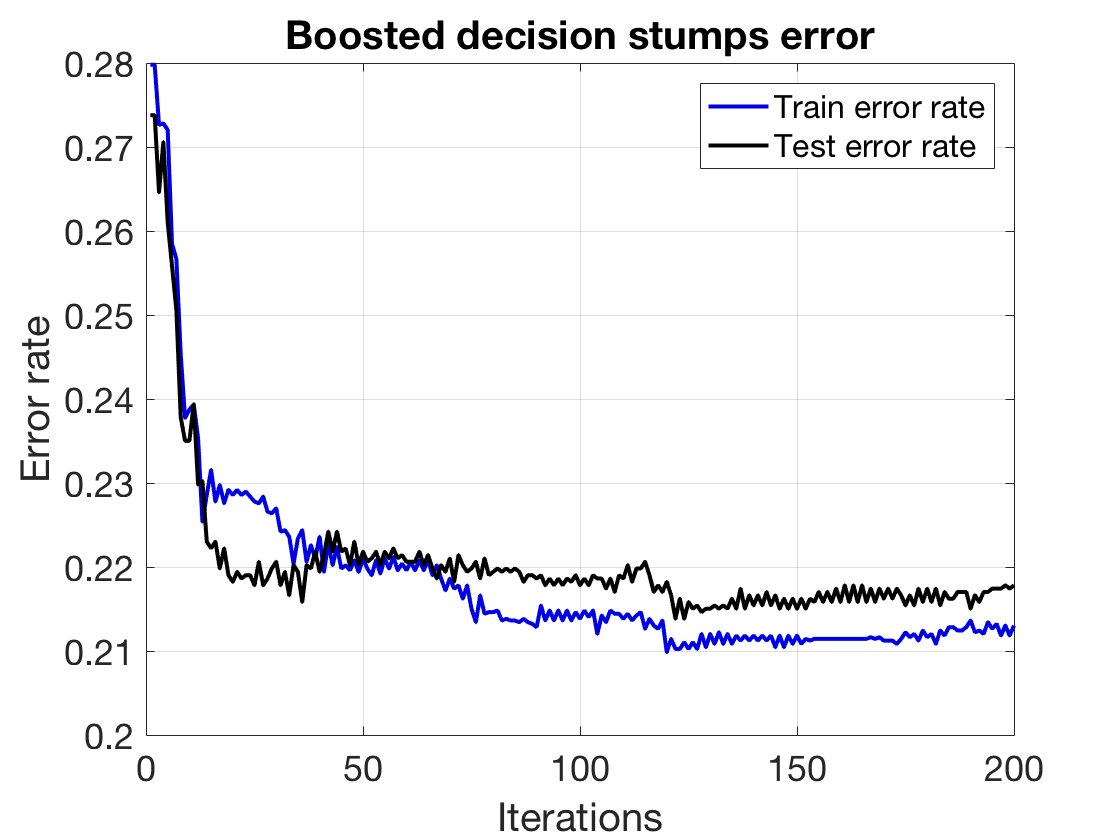
\includegraphics[width=\linewidth]{Boosted_decision}
  \caption{This is plots the error against the iterations for the regularly boosted decision stump.}
  \label{fig1:sub1}
\end{subfigure}%
\begin{subfigure}{.5\textwidth}
  \centering
  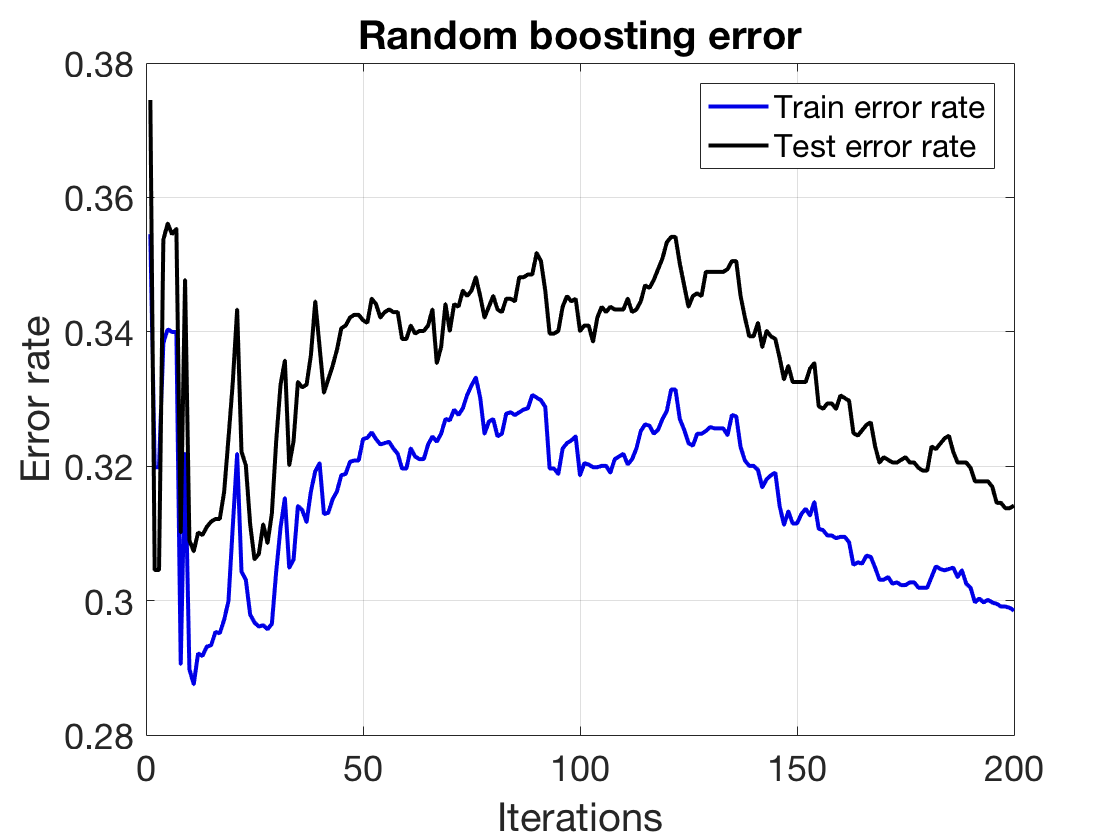
\includegraphics[width=\linewidth]{Random_boosting}
  \caption{This is plots the error against the iterations for the randomly boosted decision stump.}
  \label{fig1:sub2}
\end{subfigure}
\caption{These two figures are the error against iteration plots of the regularly and randomly boosted decision stumps, respectively. The regularly boosted decision stump significantly decreases its error rate after ~50 iterations. However, it begins to overfit for the training test set after ~50 iterations. This can be remedied by using a different scoring function rather than one that rewards over fitting. For the randomly fitted plot, the error rate decreases and increases randomly until ~50 iterations and steadily increases error until ~100 iterations where it starts to lower the error. However, it consistently overfits for the training data. Again, this can be remedied by using a different scoring method such that it discourages overfitting.}
\label{fig 1}
\end{figure}
}\label{prob:6d4}
%%% END SUBSUBSECTION 4 %%%%%%%%%%%%%%%%%%%%%%%%%%%%%%%%%%%
}\label{prob:6d}
%%% END SUBSECTION 4 %%%%%%%%%%%%%%%%%%%%%%%%%%%%%%%%%%%%%%
}\label{problem 6}
%%% END SECTION 6 %%%%%%%%%%%%%%%%%%%%%%%%%%%%%%%%%%%%%%%%%
\end{document}